\documentclass[a4paper,14pt]{article} 


\usepackage{fontenc}			
\usepackage[utf8]{inputenc}			
\usepackage[english,russian]{babel}	

\usepackage{graphicx, scalerel}    
\usepackage{wrapfig}               
\usepackage[14pt]{extsizes}        
\usepackage[warn]{mathtext}       
\usepackage{indentfirst}      
\usepackage{geometry}
\usepackage[table,xcdraw]{xcolor} 
\usepackage{amsmath,amsfonts,amssymb,amsthm,mathtools}
\usepackage{wasysym}                
\usepackage{upgreek}                
\usepackage{caption}
\usepackage{multirow}
\captionsetup{labelsep=period}
\usepackage[font=small,labelfont=bf]{caption}
\usepackage{gensymb}
\usepackage[unicode, pdftex]{hyperref}
\usepackage{fancyhdr}
\setlength\fboxsep{3pt}
\setlength\fboxrule{1pt}
\usepackage{tocloft}
\usepackage[pdftex]{lscape}
\usepackage{icomma}
\setlength{\arrayrulewidth}{0.4mm}
\usepackage{setspace}
\usepackage{pdfpages}
\usepackage{cmap}

\graphicspath{pictures/}


\newcommand{\tocsection}[1]{\section*{#1} \addcontentsline{toc}{section}{#1}}
\newcommand{\tocsubsection}[1]{\subsection*{#1} \addcontentsline{toc}{subsection}{#1}}
\renewcommand{\cftsecleader}{\cftdotfill{\cftdotsep}}

\newcommand{\comment}[1]{}


\geometry{a4paper,
		  total={170mm,257mm},
		  left=30mm,
		  right=15mm,
		  top=20mm,
		  bottom=20mm}
\onehalfspacing
\setlength{\parindent}{12.5mm}

\bibliographystyle{plain}


\begin{document}
	\newcommand{\HRule}{\rule{\linewidth}{0.7mm}}

\begin{center}
	\large\textbf{Московский Физико-Технический Институт}\\
	\vfill
		
	\Large Микроархитектура современных микропроцессоров
	\\[0.4cm]
	{ \huge \bfseries Replacement Policies}
	\\[0.4cm]
	
	\ \\
	\textbf{\large Автор:} \\	
	\large Овсянников Михаил\\
	\vfill
	\large Долгопрудный, 2025
\end{center}

\thispagestyle{empty}

\newpage
\setcounter{page}{2}

	
	\section*{Предсказатели переходов}

	В качестве первого задания необходимо было исследовать различные предсказатели переходов (branch predictors). Для бенчмаркинга использовался симулятор \href{https://github.com/ChampSim/ChampSim}{ChampSim} и некоторый набор трасс SPEC CPU 2017 из DPC-3, предназначенный специально для него.
	
	Для оценки производительности предсказателей использовались показатели IPC (Instructions Per Cycle) и MPKI (Mispredictions Per Kilo Instruction), усредненный по всем используемым трассам с помощью геометрического среднего.
	
	Всего сравнивались три предсказателя: Bimodal Predictor, Markov Predictor и Markov Probability Predictor. Ниже представлены результаты замеров IPC бенчмарков. Заметно, что Bimodal лучше Markov, а он в свою очередь -- лучше Markov Probability. 
	
	\begin{figure}[h!]
		\centering
		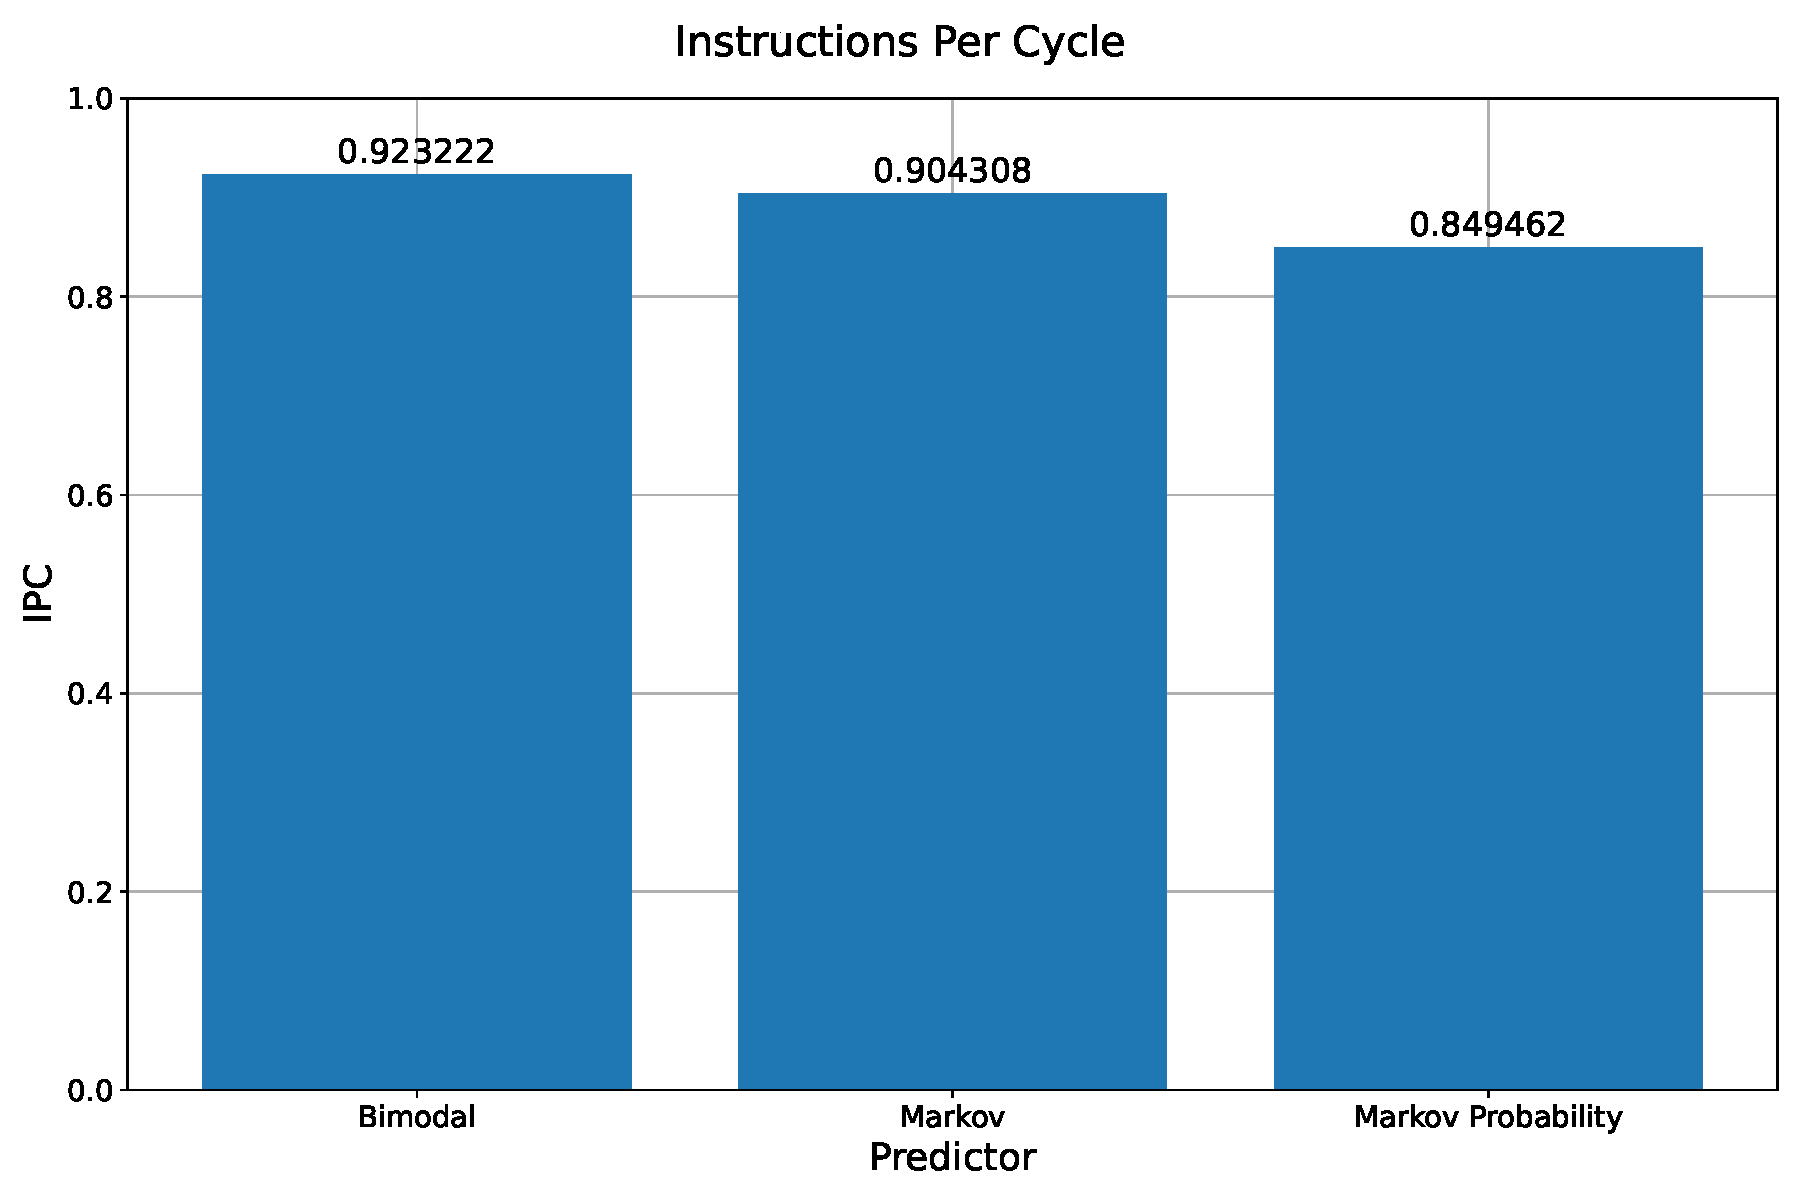
\includegraphics[width=\linewidth]{./pictures/ipc_gmean.pdf}
		\caption{IPC предсказателей}
	\end{figure}
	
	\newpage
	Увеличим масштаб, чтобы более детально рассмотреть отличия.

	\begin{figure}[h!]
		\centering
		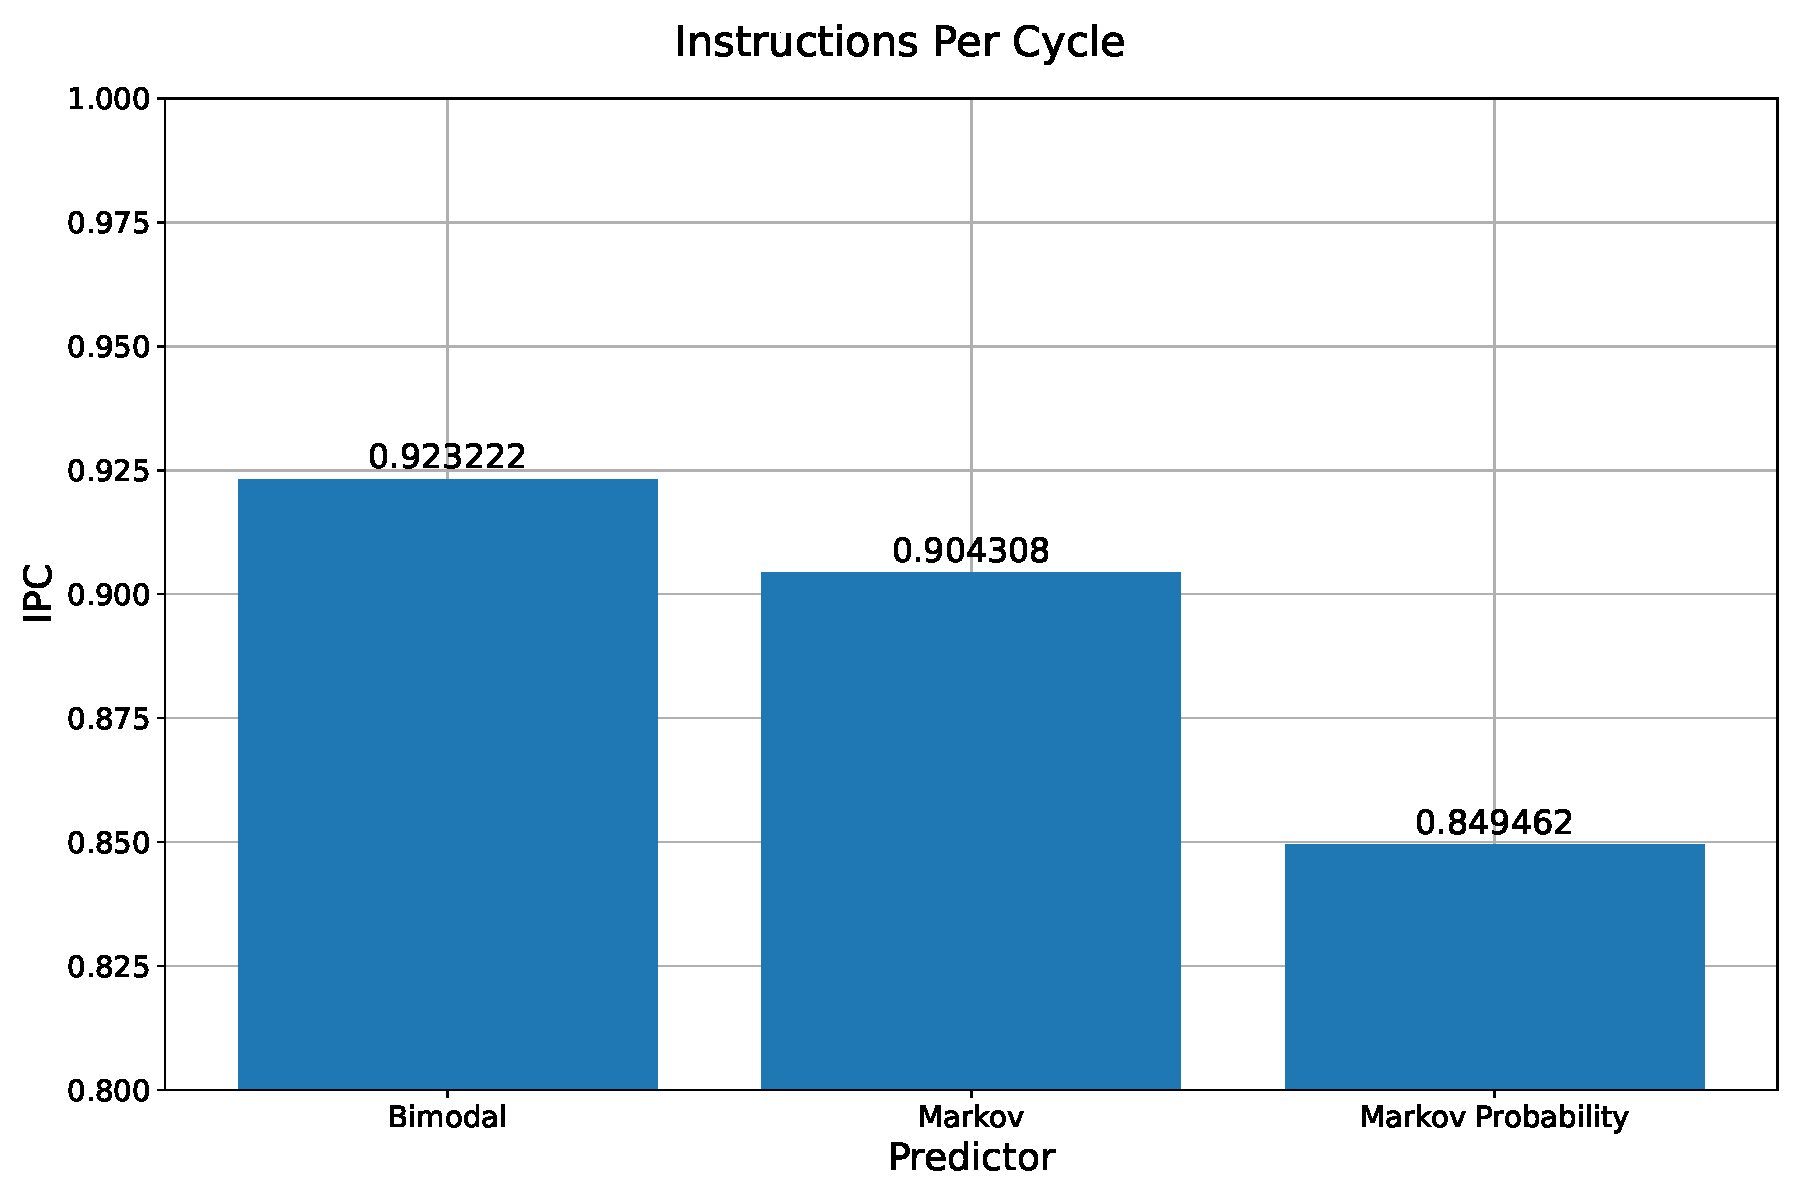
\includegraphics[width=\linewidth]{./pictures/ipc_gmean_zoomed.pdf}
		\caption{IPC предсказателей (увеличено)}
	\end{figure}

	\newpage
	Теперь посмотрим на показатели MPKI для предсказателей
	\begin{figure}[h!]
		\centering
		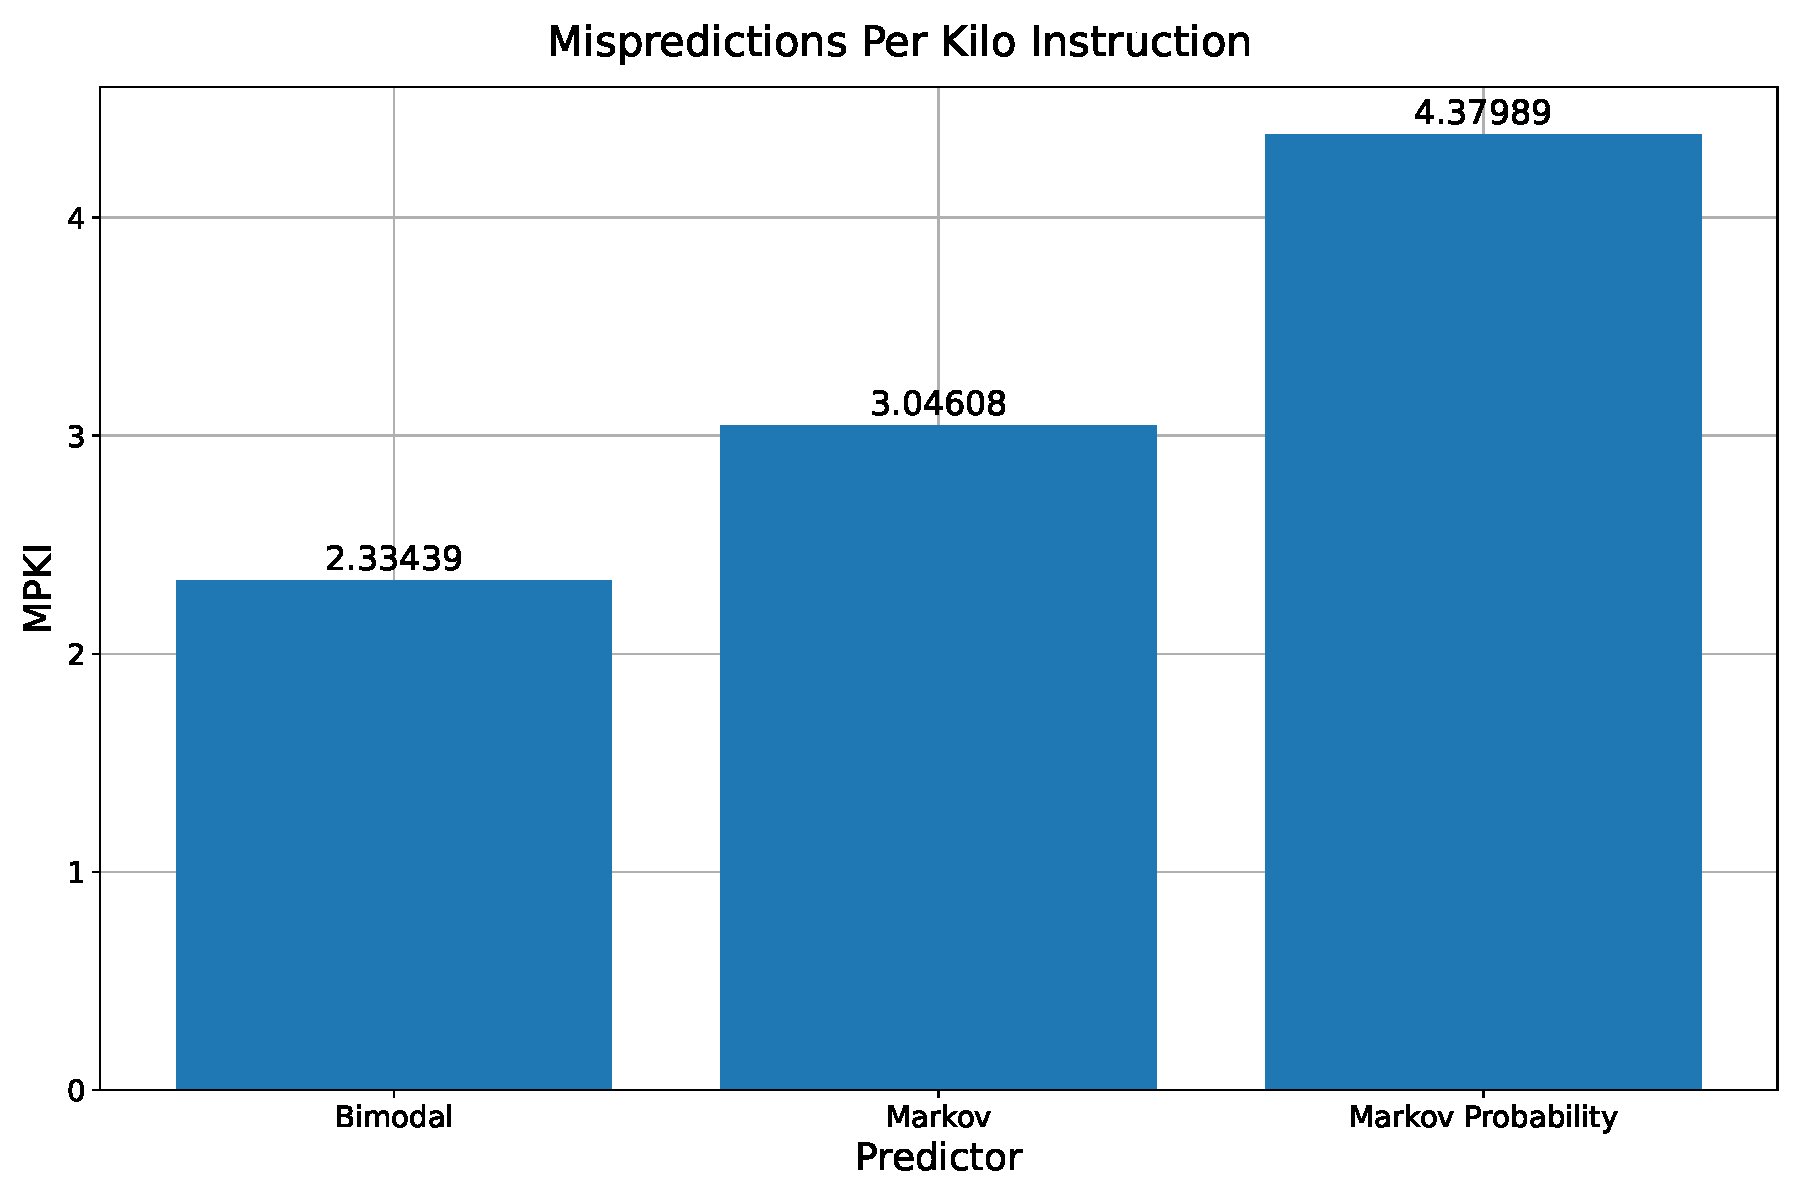
\includegraphics[width=\linewidth]{./pictures/mpki_gmean.pdf}
		\caption{MPKI предсказателей}
	\end{figure}
	
	Здесь видим ту же картину с точки зрения производительности: Bimodal лучше Markov, а тот -- лучше Markov Probability.
	
	Одно из объяснений, почему так происходит, заключается в том, что Bimodal Predictor в реализации имеет счётчики с насыщением. Причём, количество состояний этих счётчиков довольно мало. Благодаря этому данный предсказатель имеет низкую инерционность -- он быстро подстраивается под новую фазу программы с новым поведением переходов. В то же время Markov и Markov Probability предсказатели оперируют обычными счётчиками, ничем не ограниченными, поэтому при изменении поведения переходов в программе они дольше будут подстраиваться под них.
	
	Markov Probability выдаёт показатели хуже, чем просто Markov, потому, что периодически он предсказывает противоположный от него результат. В период перестройки счётчиков, когда программа меняет поведение, это оправдано, поскольку таким образом снижается негативный эффект инерционности Markov предсказателя. Однако в остальное время данное свойство лишь ухудшает картину.
	
	\newpage
	
	\section*{Вывод}
	В этом задании были исследованы различные предсказатели переходов. Проведено сравнение следующих трёх: Bimodal Predictor, Markov Predictor и Markov Probability Predictor. По результатам бенчмаркинга оказалось, что Bimodal лучше Markov, а он в свою очередь -- лучше Markov Probability.

\end{document}